\chapter{Experiment}
\label{ch:experiment}

(TODO RAAMWERK) Indien een bepaald framework boven een bepaalde scoregrens ligt zal deze worden opgenomen in het experiment.
Voor het experiment zal een simpele applicatie worden ontwikkelt (touch op het scherm creëert een object) voor elk framework a.h.v. deze applicatie zullen dan volgende kenmerken worden gemeten:  FPS, memory usage.

Indien ik informatie vindt over het automatisch testen van AR applicaties zal deze ook hier terecht komen. Ook zal dit een invloed hebben op het uitvoeren van de experimenten. Als ik hierover bruikbare informatie vind zal ik deze ook gebruiken om het experiment meerdere malen uit te voeren i.p.v. het gelimiteerde aantal keren indien ik het manueel moet doen.

\section{Afbeeldingsherkenning}
Elk framework zal ook een lijst krijgen van 10 afbeeldingen om te kijken hoe goed hij verschillende afbeeldingen kan herkennen. Hier zal er ook worden gekeken van hoever hij deze kan herkennen!
Een conclusie waarom bepaalde afbeeldingen niet worden herkent kan hier ook in komen
\begin{figure}
    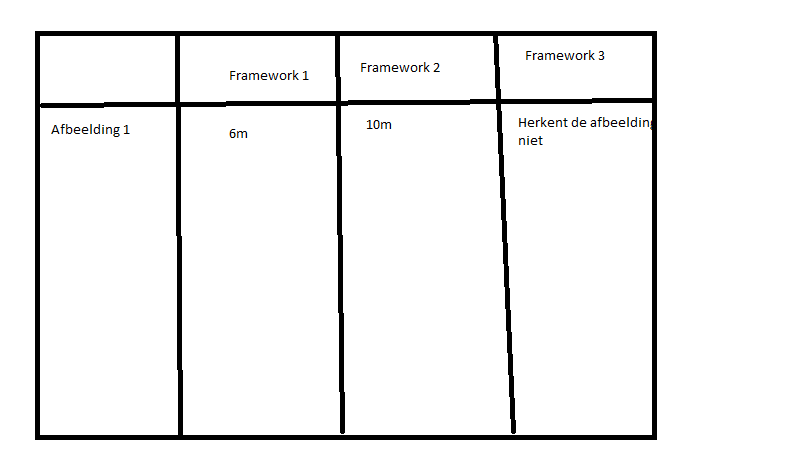
\includegraphics[width=\textwidth]{img/imgrex}\caption{Tabel aantal meter tot herkenning}\label{fig:imgrex}
\end{figure}

\section{FPS}\label{sec:fps}

Uit de data van beide frameworks blijkt het dat Vuforia maximum 60 FPS kan halen terwijl ARCore maar een maximum behaalt van 30 FPS. Het halen van een 60 FPS is redelijk onbelangrijk omdat vele Android Smartphones (vooral de iets oudere) nog geen 60 FPS camera ondersteunen. Het belangrijkste is een constant framerate behouden zonder veel grote FPS drops.

Om na te kijken of het framework een constant framerate kan behouden wordt de standaardafwijking gebruikt. Een kleine standaardafwijking wijst er namelijk op dat de datapunten weinig afwijken van het gemiddelde.

\begin{itemize}
    \item Vuforia: 1,60
    \item ARCore: 1.03
\end{itemize}

Beide frameworks hebben een kleine standaardafwijking wat er op wijst dat hun framerate redelijk (maar niet honderd procent) constant is. 

Een standaardafwijking groter dan nul wijst erop dat data niet constant is. Bij beide frameworks zijn er dus FPS drops aanwezig.

De grote van de FPS drops hebben een grotere impact op de ervaring dan de frequentie van de drops. Kleine drops van één tot twee frames hebben geen impact op de ervaring voor gebruiker omdat ze niet zichtbaar zijn. Daarom analyseert deze studie alleen maar de FPS drops die groter zijn dan tien frames.

\begin{itemize}
    \item Vuforia: 5
    \item ARCore: 3
\end{itemize}

\subsection{Analyse FPS Drops: Vuforia}

De oorsprong van de FPS drops bij Vuforia is makkelijk te achterhalen door naar het tijdstip te kijken wanneer ze voorkomen (zie tabel \ref{tbl:vuforiadrop}). In deze tabel is duidelijk te zien dat de drops altijd voorkomen bij het opstarten van de applicatie.

\begin{table}[]
    \begin{tabular}{@{}l|l|l|l|l|l@{}}
        & Drop 1   & Drop 2   & Drop 3   & Drop 4   & Drop 5   \\ \midrule
        Experiment         & 1        & 2        & 3        & 4        & 5        \\
        Tijdstip           & 1.003758 & 1.015506 & 1.013395 & 1.012443 & 1.012150 \\
        Frames per seconde & 33       & 34       & 32       & 34       & 34      
    \end{tabular}
    \caption{Oorsprong FPS drops experiment Vuforia}\label{tbl:vuforiadrop}
\end{table}

Op figuur \ref{fig:vuforiaTimeDrop} is te zien dat de framerate voor het verdere verloop van de applicatie stabiel blijft met hier en daar een kleine FPS (minder dan 10 frames) drop.

\begin{figure}
    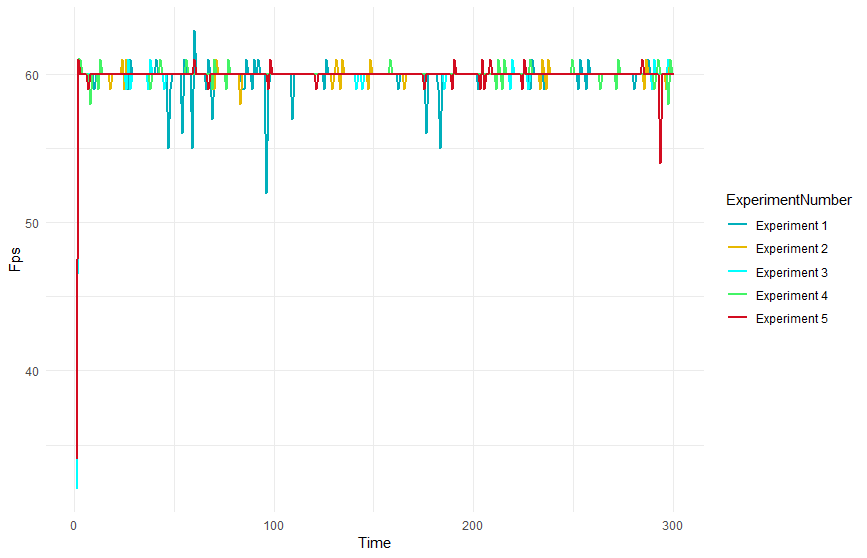
\includegraphics[width=\linewidth]{vuforiaTimeDrop.png}
    \caption{Vuforia: verloop van de FPS bij alle experimenten}
    \label{fig:vuforiaTimeDrop}
\end{figure}

\subsection{Analyse FPS Drops: ARCore}
Hoewel ARCore minder drops heeft dan Vuforia zijn ze wel veel groter (zie tabel \ref{tbl:arcoredrop}) in secties \ref{sec:memory} en \ref{sec:gameobjects} worden de oorzaken van deze drops verder besproken. Op figuur \ref{fig:arcoreTimeDrop} is te zien dat net zoals bij Vuforia de FPS bij alle experimenten redelijk consistent blijft doorheen de applicatie. Het grote verschil met Vuforia is dat de kleinere drops hoofdzakelijk geconcentreerd zijn in het begin (eerste 50 seconden) in plaats van verspreid te doorheen de looptijd van de applicatie. 

\begin{table}[]
    \begin{tabular}{@{}l|l|l|l@{}}
        & Drop 1    & Drop 2   & Drop 3    \\ \midrule
        Experiment         & 2         & 4        & 4         \\
        Tijdstip           & 218.63180 & 85.33646 & 250.73920 \\
        Frames per seconde & 8         & 7        & 10       
    \end{tabular}
    \caption{Oorsprong FPS drops experiment ARCore}\label{tbl:arcoredrop}
\end{table}

\begin{figure}
    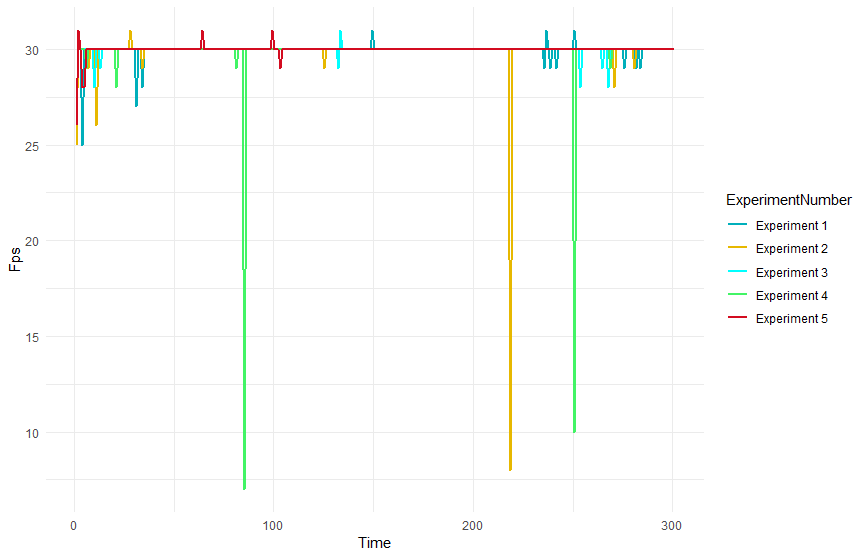
\includegraphics[width=\linewidth]{arcoreTimeDrop.png}
    \caption{ARCore: verloop van de FPS bij alle experimenten}
    \label{fig:arcoreTimeDrop}
\end{figure}

\section{RAM}\label{sec:memory}
Door de gemiddelden en standaardafwijkingen van het gereserveerde en geallorceerde RAM van beide frameworks te berekenen is het duidelijk dat de ARCore applicatie gemiddeld 4MB minder RAM verbruikt dan Vuforia. Dit is ook makkelijk te bewijzen door aan beide datasets een kolom toe te voegen waarin staat tot welk framework ze behoren en deze datasets samen te voegen. Op deze nieuwe dataset is een t-test uitgevoerd die als resultaat een p-waarde van 1 had wat erop wijst dat er een sterk verband is tussen het gekozen framework en het verbruikte RAM.

Het RAM-verbruik van Vuforia fluctueert ook veel meer dan ARCore, een standaardafwijking van 4.5MB tegenover 0.06MB. Dit is ook te bewijzen door een t-test uit te voeren op een nieuwe kolom die het vorige RAM - het huidige RAM bevat. Het resultaat van deze test was een p-waarde van 0.7419 wat aantoont dat het RAM-verbruik van ARCore inderdaad stabieler is.

Wanneer het gereserveerde RAM stijgt is het ook logisch dat gealloceerde RAM stijgt. Een applicatie gaat niet meer RAM reserveren tenzij deze meer RAM nodig heeft. Dit is bewezen door het correlatiecoëfficiënt van gereserveerd tegenover gealloceerd RAM en het correlatiecoëfficiënt van de stijging in gereserveerd RAM tegenover de stijging in gealloceerd RAM te berekenen. In tabel \ref{tbl:ramcor} is te zien dat bij beide frameworks hier een volstrekt verband is.

\begin{table}[]
    \begin{tabular}{@{}l|l|l@{}}
        & Gereserveerd tegenover gealloceerd & Stijging gereserveerd tegenover stijging gealloceerd \\ \midrule
        Vuforia & 0.9987308                          & 0.9496204                                            \\
        ARCore  & 0.9981332                          & 0.9999941                                           
    \end{tabular}
 \caption{De correlatiecoëfficiënten gereserveerd en gealloceerd RAM tonen een duidelijk verband}
\end{table}

\subsection{Correlatie RAM en FPS}
Zoals er eerder vermeld in sectie \ref{sec:fps} kampen beide frameworks met FPS drops. Om deze FPS drops te verklaren 


\section{Conclusie best scorend framework}
Hierin komt de conclusie over het best scorend framework en waarom deze de best scorende is. Hierin zal ook rekening worden gehouden met de score van het vorige hoofdstuk!